The large scale structure of our local universe is dominated by voids and filamentary structures of groups and clusters of galaxies 
(e.g., Courtois et al.\ 2013).  Half of the Local Volume galaxies reside in loose groups and associations, such as the Sculptor filament 
and the Canes Venatici Cloud (Karachentsev 2005). The nearest such structure is the NGC~3109 association (see Figure 1), an
 association of 5 dwarf galaxies in Leo, Sextans, and Antlia (van den Bergh 1999; Tully et al.\ 2006). This galaxy association, 
 with a linear extent of 1.2~Mpc across the sky (Bellazzini et al.\ 2013), lies just at the edge of the Local Group at a distance of 
 1.3--1.7 Mpc. Pawlowski \& McGaugh (2014) identified several possibilities for the origin of the NGC~3109 association: 
  an infalling dark matter filament, a  pre-existing group tidally stretched by an encounter with the MW, or galaxies
 formed as tidal dwarfs from a past Milky Way/M31 encounter. Constraining the number and properties  of additional group
 members can help to discriminate between these possibilities. The search for additional group members
 also has implications for predictions from Local Volume simulations that  at least a dozen more dwarf galaxies 
 outside the virial radii of M31 and the Milky Way  remain to be discovered (Garrison-Kimmel et al.\ 2014).
 
Recent discoveries of  the newest member of the NGC~3109 association, Leo P (Giovanelli et al.\ 2013),
and tidal substructure near the Antlia dwarf suggestive of an interaction with NGC~3109 (Penny et al.\ 2012)
mean that the time is right for a search for additional members of the association. While the region is covered by existing  and planned
survey data, none are deep enough to detect  faint galaxies and  structures at this distance. The most
well-known recent examples of nearby dwarf galaxy discovery are from the SDSS (e.g., Koposov et al.\ 2008).
Despite lying within the SDSS footprint, Leo P was discovered as part of a blind H~I survey; it is too faint to
be well-detected at the SDSS  depth ($g=22.2$, $i=21.3$), and
using LBT imaging, McQuinn et al.\ (2013) measured the tip of its red giant branch to be at $i=22.1$.
A wide-field optical survey has the potential to detect
additional  faint members of the group as well as tidal debris from interactions between members.


The outcome of a search for additional members of the NGC~3109 association has  implications for
understanding galaxy evolution. A lack of additional tidal debris would constrain the timescales and 
progenitor galaxy masses involved in a tidal dwarf origin.
A lack of additional bound-galaxy members of the group  would constrain the mass of a possible dark-matter filament or progenitor halo.
On the other hand, finding additional members of the group and subsequent follow-up would allow a better characterization of 
the group's spatial and kinematical extent; current studies  suffer from small-number statistics. If additional group members lie close to the same plane
as the existing members, this would tend to confirm Pawlowski \& McGaugh's (2014) claim
that the non-satellite galaxies to the north of the Milky Way are confined to a single plane.
Identification of new members as potential `backsplash galaxies' (Teyssier et al.\ 2012) or not  could also test
Pawlowski \& McGaugh's claim that there is an `overabundant backsplash galaxy' problem with $\Lambda$CDM.
Additional group members  would also allow better constraints on the group's  luminosity function and subsequent comparison to CDM 
simulations of galaxy formation in  low-density environments (as in Garrison-Kimmel et al. 2014).
Using a Local Group formation simulation, Ben{\'{\i}}tez-Llambay et al.\ (2013) suggested that gas removal through 
stripping by the `cosmic web' of filaments and pancakes could explain the diversity of properties of local dwarf galaxies;
identification of additional galaxies possibly associated with a filament could provide additional tests of this idea.
Finally, the tidal-dwarf characterization of the group can be tested with follow-up spectroscopy in order to determine
whether additional group members are dark-matter dominated.

We propose here to map the northern portion of  the NGC~3109 filament with CFHT/MegaCam. 
Deeper imaging than the available  SDSS  data ($g=22.2$, $i=21.3$) is required in order to detect dwarf galaxies at distances beyond 1 Mpc.
CFHT/MegaCam's ability to go both wide and deep is essential for such observations: the nearby nature of the 
filament means that it covers a large area of sky, yet the expected faint dwarf galaxies are resolved into individual stars.
The area to be mapped, defined  by the direction from Leo~P to Sextans~A/B, happens to pass quite close
to the more nearby (240~kpc) Local Group dSph Leo~I. Pe{\~n}arrubia et al.\ (2009) predicted the location
of a tidal break in this galaxy's surface brightness profile which is beyond the radius currently mapped (Sohn et al.\ 2007);
the MegaCam imaging can be used to probe the outer reaches of Leo~I and test this prediction, as well as searching
for additional nearby low-surface-brightness features.

The goal of this proposal is to complete the substructure census and probe the faint end of the luminosity function in 
a portion of the nearest filamentary structure in the universe. Detected structures will be characterized in terms of 
structural properties and their association to the sub-group will be pursued via tip-of-the-red-giant-branch 
(TRGB; Lee et al.\ 1993) measurements and, where possible, spectroscopic measurements (e.g. with Gemini/GMOS). 
Multi-wavelength follow-up can be pursued with the ALFALFA H{\sc i} survey and other wide-area surveys.
The key first step is identifying additional NGC~3109 group galaxies, for which MegaCam is
ideally suited.


\begin{figure}
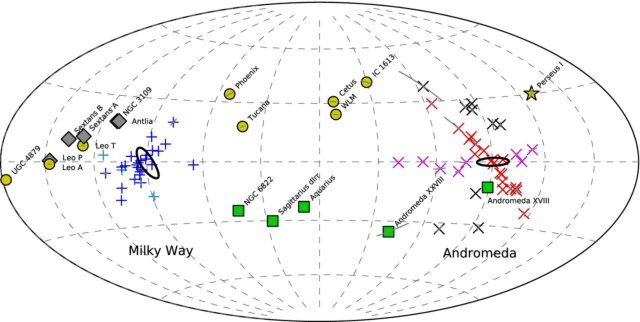
\includegraphics[scale=0.9]{pm14_fig2}
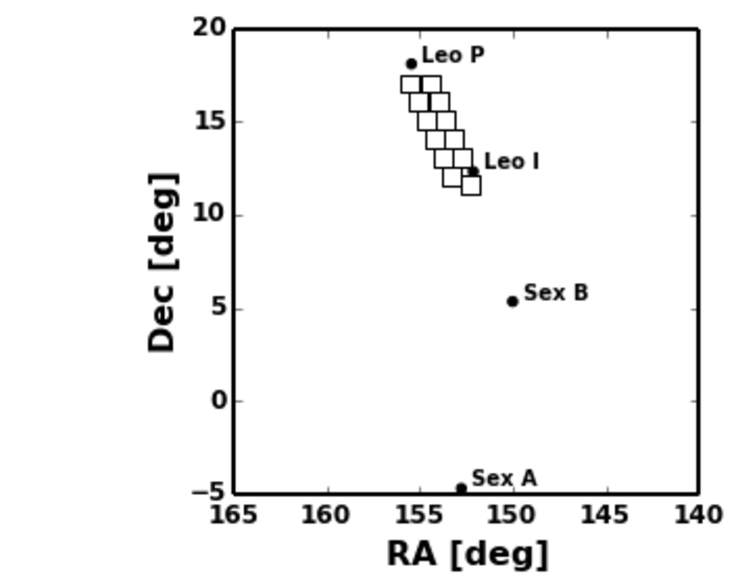
\includegraphics[scale=0.6]{fields_leoi_new}
\caption{(Left)  From Pawlowski \& McGaugh (2014): Local Group galaxies on the sky as seen from a position half-way between M31 and the Milky Way.
The NGC 3109 association members are shown as grey diamonds.
(Right) Sky projection of the proposed observations. The boxes are 1-degree MegaCam fields; the black circles at the galaxy
locations have 15-arcminute radii. 
}
\end{figure}



\section*{References}

{\small
\begin{table}[h]
\begin{tabular}{ll}
Bellazzini, M. et al.\  2013, A\&A 559, L11                 &          Lee, M.G. et al.\ 1993, ApJ, 417, 993 \\ 		    
Bellazzini, M. et al.\  2014, A\&A 566, 44 		    &		McQuinn, K.B.W. et al. 2013, AJ, 146, 145\\				    
Ben{\'{\i}}tez-Llambay, A. et al. 2013, ApJ, 763, L31	    &		Pawlowski, M.S. et al. 2014, MNRAS, 440, 908\\				    
Chiboucas, K. et al.\  2009, AJ, 137, 3009 		    &		Pe{\~n}arrubia, J. et al.\ 2009, ApJ, 298, 222 \\			    
Courtois, H.R. et al.\ 2013, AJ, 146, 69 		    &		Penny, S.J. et al. 2012, ApJ, 758, L32\\		    
Garrison-Kimmel, S. et al.\ 2014, MNRAS, 444, 222 & Sohn, S.T. et al.\ 2007, ApJ, 663, 960\\		
Giovanelli, R. et al.\ 2013, AJ, 146, 15 		    &		Teyssier, M. et al.\ 2012, MNRAS, 426, 1808\\				    
Karachentsev, I. 2005, AJ, 129, 178			    &		Tully, R.B. et al.\ 2006, AJ, 132, 729\\				    
Koposov, S. et al.\ 2008, ApJ, 686, 279                     &		van den Bergh, S. 1999, ApJ, 517, L97\\                                     

\end{tabular}
\end{table}
}
